\section{Approach}
\label{sec:approach}

%\KZ{Avoid repeating things already said in the intro unless it's really necessary to
%repeat and stress. People always read intro first before approach!}
Our approach divides the training for dialogue summarization into two stages: 
post-training and fine-tuning (Figure~\ref{fig:stage}). 
The model can be any seq-to-seq PLMs and remains unchanged
except for the parameters which are updated stage by stage.
In Stage 1, we construct multiple datasets based on the original dialogue summarization data.
The model learns to rephrase from dialogue utterances into
third-person narratives using the rephrasing data or the PGG task.
 In Stage 2, the model is fine-tuned by an auto-regressive
text generation task as usual using the original dataset. We will elaborate on Stage 1 in the rest of this section.


%\begin{figure}[t]
%	\centering
%	\subfigure[Overall Approach]{
%		%		\centering
%		%		\begin{minipage}[t]{0.5\linewidth}
%		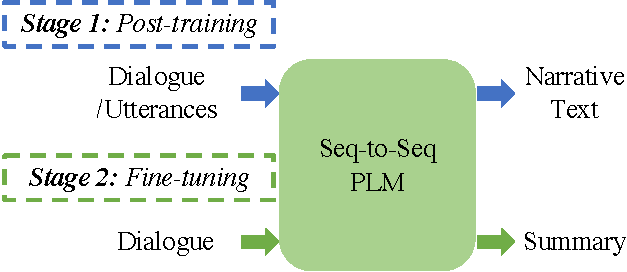
\includegraphics[scale=0.7]{stage.pdf}\label{fig:stage}
%		%		\end{minipage}
%	}
%	
%	\subfigure[PGG Task]{
%		%	\centering
%		%	\begin{minipage}[t]{0.5\linewidth}
%		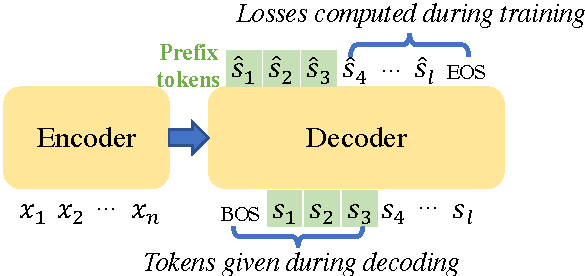
\includegraphics[scale=0.7]{pgg.pdf}\label{fig:pgg}
%		%	\end{minipage}
%	}
%	\caption{Illustrations of our overall approach and PGG task. BOS and EOS are special tokens indicating the beginning and the end of decoding.}
%	\label{fig:approach}
%\end{figure}


\begin{figure}
	\centering
	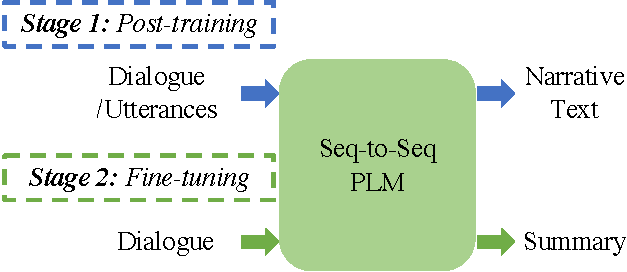
\includegraphics[width=0.8\columnwidth]{stage.pdf}
	\caption{An illustration of our approach.}
	\label{fig:stage}
\end{figure}

%\subsection{Post-training for Rephrasing} 
%The intuition for post-training is to narrow down the comprehension gap between 
%dialogue and narrative text. To this end, we post-train the model to learn the rephrasing ability, 
%as a preliminary competency for dialogue summarization. We construct rephrasing datasets in different ways and propose a new prefix-guided generation task.
%
%\KZ{An overview pic of the framework here.}

\subsection{Rephrasing Dataset Construction}
\label{sec:rephrasedata}
%Since there is no available dialogue-to-text rephrasing data as far as we know, 
We construct rephrasing datasets from the dialogue summarization dataset itself without incorporating other datasets. 
%In this way, we don't need additional efforts to collect or label external data. 
%One advantage is this kind of dataset is in the same domain as the final dialogue summarization, 
%doing away the need for domain adaptation in fine-tune stage.
%All of the data are transformed from the training and validation sets, leaving the test set untouched to avoid information leak.
The original dialogue summarization dataset (\textbf{DSum}) is made up of dialogue-summary pairs. 
A dialogue $D$ can be formalized as a sequence of $T$ turns in chronological order:
\begin{equation}
	D = \{U_1, U_2, ..., U_T\}
\end{equation}
Each turn $U_t$ generally consists of a speaker $r_t$ and corresponding utterance $u_t$ in a sequence of [$r_t$: $u_t$]. Generally, the utterances are concatenated into a sequence $X=\{x_1, x_2, ..., x_n\}$ as the input to the model. The corresponding summary $Y=\{y_1, y_2, ..., y_m\}$ consists of multiple sentences. $n$ and $m$ denote the number of tokens respectively.


\begin{table}
	\small
	\centering
	\begin{tabular}{lll}
		\toprule[1pt]
		\textbf{Datasets} & \textbf{Input} & \textbf{Output} \\
		\midrule[1pt]
		{DialIndirect} & $U_{1\sim8}$& \makecell[l]{Katarina says,``Hello, I got ...\\ we work together'' Jill says,\\``Hi :) ......  nice and sunny''}\\
		\midrule[1pt]
		{ExtSum} &$U_3$, $U_6$ & \makecell[l]{Katarina ...... a flat from Liz.\\ She will ...... after 6 pm.} \\
		\midrule[1pt]
		{ExtSumM} &$U_{3\sim6}$&\makecell[l]{Katarina ...... a flat from Liz.\\ She will ...... after 6 pm.}  \\
		\midrule[1pt]
		\multirow{2}{1cm}{{ExtSent/\\ExtSentM}}&$U_3$&Katarina ...... a flat from Liz. \\
		\cmidrule{2-3}
		& $U_6$ &Katarina will ...... after 6 pm. \\
		\midrule[1pt]
		{DSum} & $U_{1\sim8}$& \makecell[l]{Katarina ...... a flat from Liz.\\ She will ...... after 6 pm.}\\
		
		\midrule[1pt]
		\multirow{2}{1cm}{{DialSent}} & $U_{1\sim8}$ &Katarina ...... a flat from Liz. \\
		\cmidrule{2-3}
		&$U_{1\sim8}$ &Katarina will ...... after 6 pm. \\
		
		\bottomrule[1pt]
	\end{tabular}
	\caption{An illustration of post-training pairs generated from the example in Figure~\ref{fig:example}. ExtSent and ExtSentM get the same training pairs in this case.}
	\label{tab:datasets}
\end{table}


%\KZ{Replace all the quotes! And fix the English!}
%\KZ{I think it's better to give some visual examples to illustrate these several alternatives. 
%Text descriptions are too dry.}
To make the input and output carry the same amount of information, 
one way is to fix $D$ as input and convert utterances into indirect speech 
as the output. \citet{ganesh2019restructuring} restructured dialogue into text with complicated rules
%considering discourse relations among utterances for zero-shot scenarios. However, their complicated rules 
which are not released and difficult to transfer among datasets under different scenarios. Thus, we only use simple rules to convert all of the utterances into [$r_t$ says,``$u_t$''] and concatenated as the output. We call this dataset as \textbf{DialIndirect}.

Another way is fixing $Y$ as output and removing the redundant utterances in $D$ to get the rephrasing input. We take advantage of the idea of oracle extraction for news summarization~\cite{zhou-etal-2018-neural-document} and regard the combination of dialogue utterances with the highest Rouge scores computed with $Y$ as the input. Considering that utterances are highly dependent, we modify the original extraction algorithm by extracting all of the utterances lying between the extracted ones, different from the window-sized snippet selection in~\cite{liu-etal-2021-topic-aware}.  Datasets with or without this modification are called \textbf{ExtSum} and \textbf{ExtSumM} respectively.

A summary $Y$ can be divided into sentences to get more elementary rephrasing pairs. We use Spacy~\footnote{\url{https://spacy.io/}} to do coreference resolution on $Y$ and then split it into sentences. A sentence $S = \{s_1, ..., s_l\}$ with less than $3$ words, i.e. $l<3$, are discarded since it conveys quite little information, such as ``Ally agree.''. In this way, we get the dialogue-sentence dataset (\textbf{DialSent}). Similar extraction operations can be down between $D$ and $S$, and we get \textbf{ExtSent} and \textbf{ExtSentM} datasets.
An example of different data generated from the dialogue-summary pair in Figure~\ref{fig:example} is listed in Table~\ref{tab:datasets}.





\subsection{Prefix-guided Generation Task}
Although the above extraction algorithm can balance the amount of information between $D$ and $Y$ or $S$, the coreference link within $D$ will be broken caused by such hard and explicit extraction. Since the coreference resolution tools for dialogues are as good as far narrative texts as mentioned in~\citet{liu2021coreference}, we do not do it on dialogues. 

Instead, we propose a prefix-guided generation task for data with unbalanced information volume, inspired by content planning works\cite{narayan2021planning,wu-etal-2021-controllable}. 
%which assign a sequence of keywords to the decoder for controllable summaries during inference time.
We take the first few tokens of $S$ or $Y$ as the known prefix to the decoder, working as a soft and implicit information selector compared to extraction approaches.
The model keeps on the generation process to complete the sentence in a third-person point of view and the losses are calculated between the generated tokens and reference tokens except the prefix ones as shown in Figure~\ref{fig:pgg}. 
%We determine the number of prefix tokens as the number of tokens from the beginning to the first noun or the first verb in $S$ or $Y$.
%, according to the POS tags or dependency parsing tags recognized by Spacy.
Taking $S$ as an example, the mathematical illustration is as follows.

\begin{figure}
	\centering
	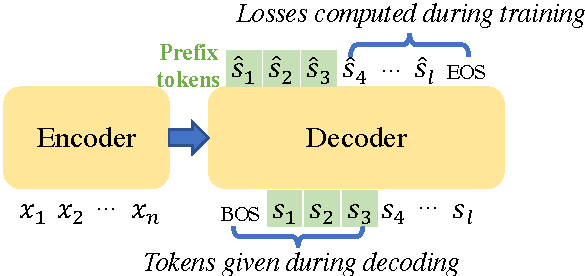
\includegraphics[width=0.9\columnwidth]{pgg.pdf}
	\caption{PGG task. BOS and EOS are special tokens indicating the beginning and the end of decoding.}
	\label{fig:pgg}
\end{figure}

The sequence-to-sequence model is made up of a bidirectional transformer encoder and an auto-regressive transformer decoder. The encoder takes the token sequence of $D$ as input and maps it into distributed representations $H^d$. The decoder takes $H^d$ as input and factorizes the probability of $S$ into the product of the conditional probability of each token. 
Our prefix-guided training task is to minimize the negative log-likelihood of $S$:
\begin{equation}
	\begin{aligned}
		L &= -\frac{1}{l-a}\sum_{t=a}^{l}\log P(s_t|s_{<t},H^d) \\
		%i &\sim U(a,b)
	\end{aligned}
\end{equation}
where $a$ is the number of prefix tokens.

During inference, the first $b$ tokens are provided for the decoder. 
We map the hidden states into a vocabulary distribution at each decoding step:
%\KZ{Is it common to refer to the decoding function as $Dec$? Function names shouldn't be
%capitalized?}
%\begin{align}
%P(\hat{s}_t|s, \hat{s}, b, t, H^d)= &\softmax(W_v{\rm Dec}(s_1,\ldots, s_b,\notag \\
%&\hat{s}_{b+1},\ldots,\hat{s}_{t-1}, H^d))
%&P(\hat{s}_t|s_{\leq b}, \hat{s}_{>b,<t},H^d)=\\
%&\softmax(W_v{\rm Dec}(s_1,\ldots, s_b, \hat{s}_{b+1},\ldots,\hat{s}_{t-1}, H^d))
%\end{align}

\begin{align}
		&P(\hat{s}_t|s_{\leq b}, \hat{s}_{>b,<t},H^d) =\\
		& \softmax(W_v{\rm Dec}(s_1,..., s_b,\hat{s}_{b+1},...,\hat{s}_{t-1}, H^d))\notag
\end{align}
%i.e. $t>k$ in Equation \ref{eq:decoder}.
where $Dec(\cdot)$ represents the decoder and decoding starts at the $b$+$1$-th token. We use POS tags (``PROPN''\&``NOUN'' or ``VERB'') or dependency parsing tags (``nsubj''\&``nsubjpass'' or ``ROOT'') by Spacy to locate the noun or verb in $S$ or $Y$ and designate $a$ sample by sample during training. For inference without knowing the ground truth of generation, we simply set $b$ as a constant equaling $4$.
%$k$ can be either equal to $a$ or simply set to a constant.

%$a$, $b$ and $k$ are hyper-parameters assigned as $\{2,4,3\}$ respectively.
In a word, the post-training stage is done by the vanilla auto-regressive generation task with DialIndrect, ExtSum, ExtSumM, ExtSent or ExtSentM dataset, or by the PGG task with DialSent or DSum.


%\subsection{Fine-tuning for Dialogue Summarization}
%
%The post-trained model can be further directly finetuned on dialogue summarization datasets to learn content selection abilities and generate a coherent summary.
%%under different scenarios and granularities.% depending on datasets. 
%%The dialogue and corresponding summary are represented as $X =\{x_1, x_2, ..., x_p\}$ and $Y=\{y_1, y_2, ..., y_q\}$, where $p$ and $q$ denote the number of tokens in the dialogue and summary. 
%We adopt the vanilla auto-regressive generation task with original dialogue-summary pairs.
%and the loss function as follow:
%\begin{equation}
%	\begin{aligned}
%		&h_1, h_2, ..., h_p = Enc(x_1, x_2, ..., x_p)\\
%		P(y_t|y_{<t},&H) = Softmax(W_vDec(y_1, ..., y_{t-1}, H))\\
%		&L = -\frac{1}{q}\sum_{t=1}^{q}\log P(y_t|y_{<t},H)
%	\end{aligned}
%\end{equation}
%where $H=\{h_1, h_2, ..., h_p\}$ represents the hidden states generated by the transformer encoder $Enc(\cdot)$.

